\section{Sztuczne sieci neuronowe}
\label{sec:artificial-neural-networks}

Sztuczne sieci neuronowe są fundamentalnym elementem głębokiego uczenia (ang. deep learning). Są to modele matematyczne, które można widzieć jako złożenie wielu nieliniowych funkcji. Idea przepływu danych jest inspirowana strukturą ludzkiego mózgu.

Sieci neuronowe składają się z dużej liczby połączonych ze sobą węzłów obliczeniowych zwanych neuronami. W uczeniu maszynowym dendryty neuronów określane są jako dane wejściowe, a jądro przetwarza dane i przekazuje obliczone dane wyjściowe przez akson. Mówiąc najprościej, sieci neuronowe reprezentują połączone jednostki wejściowe i wyjściowe, w których każde połączenie ma powiązaną wagę.

Pierwszy model neuronu został opisany przez dwóch badaczy Uniwersytetu Chicago, mianowicie neurofizjologa Warrena McCullocha i matematyka Waltera Pittsa w 1943~\cite{mcculloch1943}. Sztuczny neuron McCullocha-Pittsa jest klasyfikatorem binarnym, który dąży się do przyporządkowania danego sygnału wejściowego do jednej z dwóch klas. Neurony mogą być tylko w dwóch stanach, aktywne albo
nieaktywne. Model ten ma ograniczone możliwości uczenia, ale może być używany do rozpoznawania prostych wzorców i wykrywania podstawowych cech danych.

\subsection{Perceptron}
\label{subsec:perceptron}

W roku 1958 Frank Rosenblatt opublikował artykuł, w którym perceptron ujrzał światło dzienne~\cite{rosenblatt1958}. Perceptron jest najprostszą siecią neuronową o pojedynczej warstwie. W swojej implementacji składa się z niezależnych neuronów McCullocha-Pittsa. Mimo swojej prostoty ten model ma szerokie zastosowanie w wielu rozwiązywaniu problemów współczesnej sztucznej inteligencji, takich jak generalizacja danych, regresja, klasyfikacja, tworzenie skojarzeń i wiele innych.

Na początku perceptron przyjmuje zestaw wartości wejściowych, które są przypisane do wag. Wejścia te mogą reprezentować różne cechy lub atrybuty danych, na przykład piksele na obrazie. Każdemu wejściu przypisywane są wagi, które określają, jak bardzo dane wejście wpływa na wynik perceptronu. Wagi te są początkowo inicjowane losowo lub przy użyciu pewnej strategii uczenia. Perceptron oblicza sumę ważoną wejść, mnożąc każde wejście przez odpowiadającą mu wagę i sumując te wyniki.

Wynik sumy ważonej jest przekazywany przez funkcję aktywacji. Funkcja ta jest odpowiedzialna za ustalenie, czy perceptron powinien zostać aktywowany. Wynik działania funkcji aktywacji jest wyjściem perceptronu.

\begin{figure}[H]
    \centering
    \begin{subfigure}[H]{0.49\textwidth}
        \centering
        \begin{tikzpicture}
            \begin{axis}[
                    axis background style=white,
                    axis lines=middle,
                    xmin=-1.5,
                    xmax=1.5,
                    ymin=-1.5,
                    ymax=1.5,
                    xlabel={$x$},
                    ylabel={$f(x)$},
                    xtick={-1, 0, 1},
                    ytick={-1, 0, 1},
                    grid=major,
                ]
                \addplot[very thick, validation, domain=-2:0] {0};
                \addplot[very thick, validation, domain=0:2] {1};
            \end{axis}
        \end{tikzpicture}
        \caption{
            $f(x)=\begin{cases}
                    0 & \text{jeżeli}\,x < 0    \\
                    1 & \text{jeżeli}\,x \geq 0
                \end{cases}$
        }
        \label{fig:discrete-unipolar}
        \vspace{1cm}
    \end{subfigure}
    \hfill
    \begin{subfigure}[H]{0.49\textwidth}
        \centering
        \begin{tikzpicture}
            \begin{axis}[
                    axis background style=white,
                    axis lines=middle,
                    xmin=-1.5,
                    xmax=1.5,
                    ymin=-1.5,
                    ymax=1.5,
                    xlabel={$x$},
                    ylabel={$f(x)$},
                    xtick={-1, 0, 1},
                    ytick={-1, 0, 1},
                    grid=major,
                ]
                \addplot[very thick, validation, domain=-2:0] {-1};
                \addplot[very thick, validation, domain=0:2] {1};
            \end{axis}
        \end{tikzpicture}
        \caption{
            $f(x)=\begin{cases}
                    -1 & \text{jeżeli}\,x < 0    \\
                    1  & \text{jeżeli}\,x \geq 0
                \end{cases}$
        }
        \label{fig:discrete-bipolar}
        \vspace{1cm}
    \end{subfigure}
    \caption{Dyskretne funkcje aktywacji}
    \label{fig:discrete-activation-functions}
\end{figure}

\begin{figure}[H]
    \centering
    \begin{subfigure}[H]{0.49\textwidth}
        \centering
        \begin{tikzpicture}
            \begin{axis}[
                    axis background style=white,
                    axis lines=middle,
                    xmin=-1.5,
                    xmax=1.5,
                    ymin=-1.5,
                    ymax=1.5,
                    xlabel={$x$},
                    ylabel={$f(x)$},
                    xtick={-1, 0, 1},
                    ytick={-1, 0, 1},
                    grid=major,
                ]
                \addplot[very thick, validation, domain=-2:0] {1/(1+exp(-x*5))};
                \addplot[very thick, validation, domain=0:2] {1/(1+exp(-x*5))};
            \end{axis}
        \end{tikzpicture}
        \caption{$f(x)=\dfrac{1}{1+e^{-\lambda{x}}}$}
        \label{fig:sigmoid}
    \end{subfigure}
    \hfill
    \begin{subfigure}[H]{0.49\textwidth}
        \centering
        \begin{tikzpicture}
            \begin{axis}[
                    axis background style=white,
                    axis lines=middle,
                    xmin=-1.5,
                    xmax=1.5,
                    ymin=-1.5,
                    ymax=1.5,
                    xlabel={$x$},
                    ylabel={$f(x)$},
                    xtick={-1, 0, 1},
                    ytick={-1, 0, 1},
                    grid=major,
                ]
                \addplot[very thick, validation, domain=-2:0] {2/(1+exp(-x*5))-1};
                \addplot[very thick, validation, domain=0:2] {2/(1+exp(-x*5))-1};
            \end{axis}
        \end{tikzpicture}
        \caption{$f(x)=\dfrac{2}{1+e^{-\lambda{x}}}-1$}
        \label{fig:tanh}
    \end{subfigure}
    \caption{Ciągłe funkcje aktywacji}
    \label{fig:continuous-activation-functions}
\end{figure}

Proces uczenia perceptronu polega na dostosowywaniu wag w celu osiągnięcia poprawnej klasyfikacji danych treningowych. Algorytm uczący modyfikuje wagi w oparciu o błędy popełniane przez perceptron i dostosowuje je tak, aby lepiej dopasować się do danych treningowych.

Perceptron jest modelem liniowym i może rozwiązywać proste problemy, które są liniowo separowalne, czyli takie, w których istnieje prosty hiperpłaszczyzna dzieląca dane na dwie klasy. Dlatego też do bardziej zaawansowanych problemów używa się wielowarstwowe perceptrony z nieliniowymi funkcjami aktywacji.

\begin{figure}[H]
    \centering
    \begin{tikzpicture}
        [>=stealth]
        \node[circle, draw=black, fill=gray!30, minimum size=10mm] (sf) {};

        \draw[thick] (0.5em, 0.5em) -- (0, 0.5em) -- (0, -0.5em) -- (-0.5em, -0.5em);
        \draw(0em, 0.75em) -- (0em, -0.75em);
        \draw(0.75em, 0em) -- (-0.75em, 0em);

        \node[right=2em of sf] (y) {$y$};
        \draw[->, thick] (sf) -- (y);

        \node[circle, draw=black, fill=gray!30, minimum size=10mm, left=2em of sf] (ws) {$\sum\limits_{n=0}^{n} x_n \cdot w_n$};
        \draw[->, thick] (ws) -- (sf);

        \node[rectangle, draw=black, fill=gray!30, left=2em of ws] (w1) {$w_1$};
        \node[circle, draw=black, fill=gray!30, minimum size=10mm, left=2em of w1] (x1) {$x_1$};
        \draw[thick] (x1) -- (w1);
        \draw[->, thick] (w1) -- (ws);

        \node[below of=w1] (dots) {$\vdots$};
        \node[below of=x1] (ldots) {$\vdots$};

        \node[rectangle, draw=black, fill=gray!30, below of=dots] (wn) {$w_n$};
        \node[circle, draw=black, fill=gray!30, minimum size=10mm, left=2em of wn] (xn) {$x_n$};
        \draw[thick] (xn) -- (wn);
        \draw[->, thick] (wn) -- (ws);

        \node[rectangle, draw=black, fill=gray!30, above=2em of w1] (w0) {$w_0$};
        \node[circle, draw=black, fill=gray!30, minimum size=10mm, left=2em of w0] (1) {$1$};
        \draw[thick] (1) -- (w0);
        \draw[->, thick] (w0) -- (ws);

        \node[above=1em of 1, font=\scriptsize] {Wejścia};
        \node[above=1em of w0, font=\scriptsize] {Wagi};
        \node[above=1em of ws, font=\scriptsize, align=center] {Suma\\wag};
        \node[above=1em of sf, font=\scriptsize, align=center] {Funkcja\\aktywacji};
    \end{tikzpicture}
    \caption{Perceptron}
    \label{fig:perceptron}
\end{figure}

Podczas trenowania sieć dostosowuje wagi neuronów, aby móc przewidzieć właściwą klasę dla danych wejściowych. Analogia ta może być rozszerzona, aby opisać poszczególne warstwy w sieci neuronowej. Tworzą ją co najmniej trzy warstwy: wejściowa, ukryta i wyjściowa, przy czym warstw ukrytych może być wiele. Warstwa wejściowa przekazuje dane z neuronów tej warstwy do każdego każdego neuronu warstwy ukrytej.

Tam przede wszystkim zachodzi proces uczenia, modyfikowane są wagi i szukane są zależności między danymi. Finalnie z warstwy wyjściowej jest zwracany wynik.

\begin{figure}[H]
    \centering
    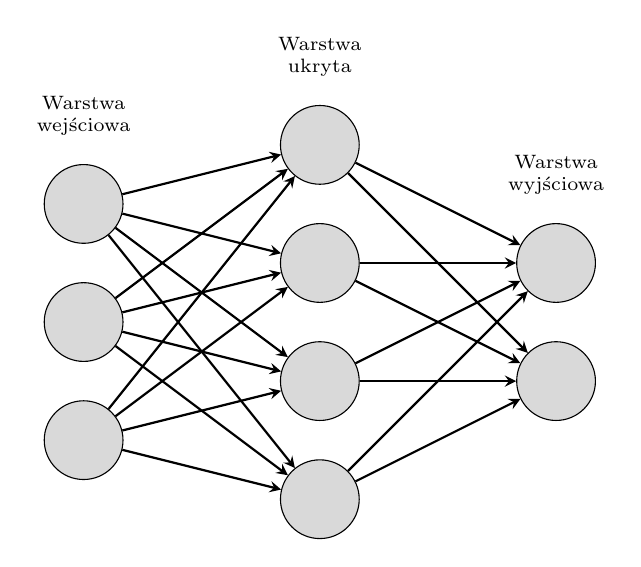
\begin{tikzpicture}
        [x=1.5cm, y=1.5cm, >=stealth]

        \foreach \i/\l[count=\y] in {1, 2, 3}
        \node[circle, draw=black, fill=gray!30, minimum size=10mm] (input-\i) at (0, 1.5-\y) {};

        \foreach \i[count=\y] in {1, 2, 3, 4}
        \node[circle, draw=black, fill=gray!30, minimum size=10mm] (hidden-\i) at (2, 2-\y) {};

        \foreach \i[count=\y] in {1, 2}
        \node[circle, draw=black, fill=gray!30, minimum size=10mm] (output-\i) at (4, 1-\y) {};

        \foreach \i in {1,...,3}
        \foreach \j in {1,...,4}
        \draw[->, thick] (input-\i) -- (hidden-\j);

        \foreach \i in {1,...,4}
        \foreach \j in {1,...,2}
        \draw[->, thick] (hidden-\i) -- (output-\j);

        \node[above, align=center, font=\scriptsize] at (0, 1.0) {Warstwa\\wejściowa};
        \node[above, align=center, font=\scriptsize] at (2, 1.5) {Warstwa\\ukryta};
        \node[above, align=center, font=\scriptsize] at (4, 0.5) {Warstwa\\wyjściowa};
    \end{tikzpicture}
    \caption{Sieć neuronowa}
    \label{fig:artificial-neural-network}
\end{figure}

\subsection{Sieci neuronowe w lingwistyce migowej}
\label{subsec:neural-networks-layers-architecture}

Największym ograniczeniem jest zbiór danych, stanowiący dane wejściowe dla modelów sieci neuronowych, stąd są różne podejścia do detekcji znaków migowych w wizji komputerowej. Istnieje wiele rodzajów sztucznych sieci neuronowych i każda ma swoje ogólne przeznaczenie oraz limity, zatem rozwiązania będą się różnić w zależności od tego, jaki problem nas dotyczy.

\subsubsection{Konwolucyjne sieci neuronowe}
\label{subsubsec:convolutional-neural-networks}

David Hubel i Torsten Wiesel badając reakcję komórek nerwowych w mózgach kotów na różne wzorce wizualne odkryli, że komórki nerwowe w korze wzrokowej reagują na konkretne kształty i cechy obrazów, takie jak linie, krawędzie i kąty. Odkrycie to przyczyniło się do zrozumienia sposobu, w jaki mózg przetwarza informacje wizualne~\cite{hubel1968}.

Sieć konwolucyjna (ang. convolutional neural network) jest inspirowana biologicznym procesem widzenia zwierząt, w którym wzorce są wykrywane przez komórki odbiorcze o ograniczonym polu receptywnym. Jej praktyczne zastosowanie dominuje głównie w dziedzinie przetwarzania obrazów i wizji komputerowej, takich jak rozpoznawanie obiektów, segmentacja obrazu, klasyfikacja schematów graficznych czy też rozpoznawanie twarzy. Dobrze wytrenowane sieci konwolucyjne mogą efektywnie rozpoznawać schematy wizualne oraz klasyfikować dane przestrzenne, w tym estymować pozę człowieka~\cite{gu2018}.

W sieciach konwolucyjnych można wyróżnić kilka podstawowych typów warstw, które są typowe dla większości architektur CNN. Te warstwy pełnią różne funkcje i są kluczowe dla przetwarzania obrazów i innych danych przestrzennych.

\begin{figure}[H]
    \centering
    \begin{tikzpicture}
        [x=1.5cm, y=1.5cm, >=stealth]

        \foreach \i [count=\y] in {1, 2, 3}
        \node[circle, draw=black, fill=gray!30, minimum size=10mm] (input-\i) at (0, 1.5-\y*1.25) {};

        \foreach \i [count=\y] in {1, 2, 3}
        \node[circle, draw=black, fill=gray!30, minimum size=10mm] (conv-\i) at (2, 1.5-\y*1.25) {};

        \foreach \i [count=\y] in {1, 2}
        \node[circle, draw=black, fill=gray!30, minimum size=10mm] (pool-\i) at (4, 0.875-\y*1.25) {};

        \foreach \i [count=\y] in {1, 2, 3}
        \node[circle, draw=black, fill=gray!30, minimum size=10mm] (fc-\i) at (6, 1.5-\y*1.25) {};

        \foreach \i in {1,...,3}
        \foreach \j in {1,...,3}
        \draw[->, thick] (input-\i) -- (conv-\j);

        \foreach \i in {1,...,3}
        \foreach \j in {1,...,2}
        \draw[->, thick] (conv-\i) -- (pool-\j);

        \foreach \i in {1,...,2}
        \foreach \j in {1,...,3}
        \draw[->, thick] (pool-\i) -- (fc-\j);

        \node[above, align=center, font=\scriptsize] at (0, 0.75) {Warstwa\\ wejściowa};
        \node[above, align=center, font=\scriptsize] at (2, 0.75) {Warstwa\\konwolucyjna};
        \node[above, align=center, font=\scriptsize] at (4, 0.25) {Warstwa\\łącząca};
        \node[above, align=center, font=\scriptsize] at (6, 0.75) {Warstwa\\wyjściowa};

    \end{tikzpicture}
    \caption{Sieć konwolucyjna}
    \label{fig:convolutional-neural-network}
\end{figure}

Warstwa konwolucyjna i warstwa łącząca są ze sobą powiązane, ponieważ warstwa konwolucyjna służy do ekstrakcji cech z danych wejściowych, a następnie warstwa łącząca redukuje rozmiar tych cech, zachowując najważniejsze informacje. Ta sekwencja warstw konwolucyjnych i warstw łączących może być stosowana wielokrotnie w sieci konwolucyjnej, co pozwala na stopniową i hierarchiczną ekstrakcję coraz bardziej złożonych cech. To z kolei umożliwia modelowi dokładniejsze rozpoznawanie i klasyfikację obiektów w danych wejściowych.

Warstwa łącząca, zwana również warstwą poolingową, jest używana do zmniejszenia wymiarów danych i zmniejszenia liczby parametrów w modelu. Jej zadaniem jest wydobycie najważniejszych informacji z mapy cech wygenerowanej przez warstwę konwolucyjną. Najczęściej stosowaną operacją łączącą jest operacja max-pooling, która działa na każdej mapie cech niezależnie. Podczas max-poolingu dzielona jest mapa cech na podregiony, a następnie wybierane jest maksymalne wartości z każdego podregionu. To sprowadza się do zredukowania rozmiaru danych i skupienia się na najbardziej istotnych cechach.

Po kilku warstwach konwolucyjnych i poolingowych często umieszcza się jedną lub więcej warstw w pełni połączonych, które przetwarzają wyniki z poprzednich warstw i wykonują końcową klasyfikację lub regresję. Warstwy w pełni połączone są podobne do warstw w tradycyjnych sieciach neuronowych.

Głównym celem CNN jest wykrywanie i ekstrakcja lokalnych cech w danych, takich jak krawędzie, tekstury i schematy. Badania w ostatnich latach nadal wykorzystują CNN do detekcji daktylografii języków migowych~\cite{rastgoo2021}. Przedstawiane rozwiązania są często bardzo precyzyjne dzięki dużej ilości zdjęć, ale wciąż są to statyczne obrazy, dlatego sprawdzi się to dla bardzo prostych znaków~\cite{cheok2019}. W samym polskim języku migowym istnieje przewaga 20 znaków dynamicznych nad 16 statycznymi.

Najbardziej oczywistym podejściem do detekcji schematów na zdjęciach lub klatkach filmu będzie użycie sieci złożonej z warstw konwolucyjnych. Jej praktyczne zastosowanie dominuje głównie w dziedzinie przetwarzania obrazów i wizji komputerowej, takich jak rozpoznawanie obiektów, segmentacja obrazu, klasyfikacja schematów graficznych czy też rozpoznawanie twarzy.

\subsubsection{Long short-term memory}
\label{subsubsec:long-short-term-memory}

LSTM (ang. long short-term memory) został wprowadzony w 1997 roku przez Seppa Hochreibera i Jürgena Schmidahubera jako rozszerzenie tradycyjnych rekurencyjnych sieci neuronowych~\cite{hochreiter1997}. W przeciwieństwie do CNN, która jest siecią jednokierunkową, LSTM jest typem sieci rekurencyjnej. Sieci jednokierunkowe to sieci neuronowe, w których sygnał przepływa tylko w jednym kierunku, od wejścia do wyjścia. W sieciach jednokierunkowych nie występuje sprzężenie zwrotne, co oznacza, że sygnał przechodzi przez każdy neuron tylko raz w swoim cyklu.

Celem stworzenia LSTM było rozwiązanie problemu znikającego gradientu, który występował w RNN i utrudniał efektywne modelowanie długoterminowych zależności w sekwencjach danych. W przypadku długich sekwencji danych, tradycyjne RNN mogą napotykać trudności propagowania informacji na długie odstępy czasowe. Informacje te mogą znikać wraz z kolejnymi krokami czasowymi.

W sieciach rekurencyjnych występuje problem znikającego gradientu, który polega na tym, że gradient błędu maleje wraz z odległością od wyjścia sieci. Aby rozwiązać ten problem, w sieciach LSTM wprowadzono dodatkowe połączenia zwane ścieżkami odwróconymi, które pozwalają na przepływ gradientu z dalszych warstw do wcześniejszych. Propagacja wsteczna (ang. backpropagation through time) to technika w uczeniu maszynowym, która pozwala na propagację gradientu błędu z dalszych warstw do wcześniejszych. W sieciach rekurencyjnych, takich jak LSTM, ta technika jest wykorzystywana do rozwiązania problemu znikającego gradientu.

Dzięki ścieżkom odwróconym gradient błędu może przejść przez całą sekwencję danych, a nie tylko przez kilka kroków czasowych. W przypadku sieci LSTM, ścieżki odwrócone pozwalają na propagację gradientu błędu przez trzy bramki LSTM (bramkę zapomnienia, bramkę wejściową i bramkę wyjściową) oraz przez stan komórki i stan ukryty. Dzięki temu sieć może uczyć się na dłuższych sekwencjach danych i uniknąć problemu znikającego gradientu. Jednostka rekurencyjna LSTM jest znacznie bardziej złożona niż jednostka RNN, co poprawia proces uczenia się, ale wymaga więcej zasobów obliczeniowych. Stan ukryty z poprzedniego kroku czasowego i dane wejściowe z bieżącego kroku czasowego są łączone i przekazywane przez różne bramki~\cite{yu2019}.

LSTM wprowadza specjalną strukturę zwaną \enquote{bramkami}, które pozwalają na kontrolowane przechowywanie i zapominanie informacji przez dłuższy czas, umożliwiając propagację gradientu na większe odstępy. Oznacza to, że LSTM ma zdolność do przechowywania ważnych informacji przez dłuższy okres czasu. Dzięki temu może nauczyć się identyfikować i przechowywać znaczące cechy o długich sekwencjach danych, co jest szczególnie przydatne w zadaniach, takich jak rozpoznawanie mowy, tłumaczenie maszynowe lub generowanie tekstu.

\begin{figure}[H]
    \centering
    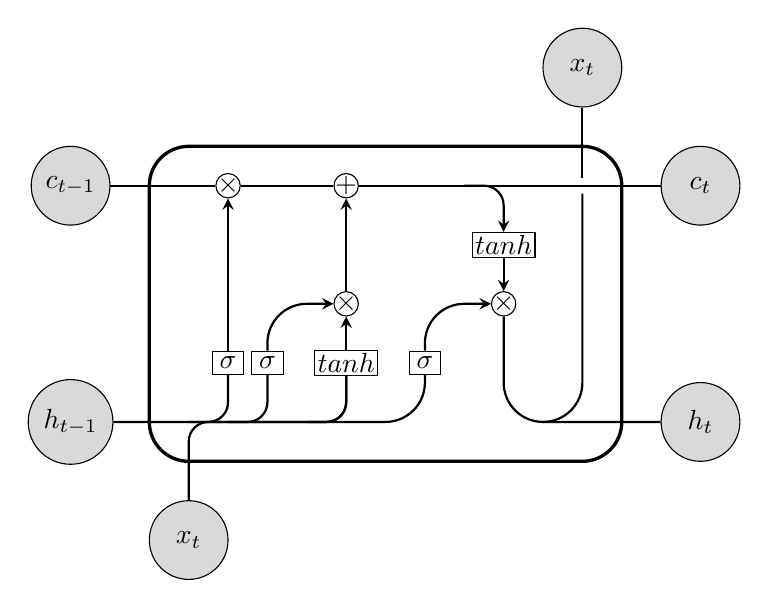
\begin{tikzpicture}
        [font=\textsf \scriptsize,>=stealth]

        \node[rectangle, rounded corners=5mm, draw=black, very thick, minimum height=4cm, minimum width=6cm] at (0, 0) {};

        \node[rectangle, draw=black, minimum width=4mm, minimum height=3mm, inner sep=1pt] (sigma1) at (-2, -0.75) {$\sigma$};
        \node[rectangle, draw=black, minimum width=4mm, minimum height=3mm, inner sep=1pt] (sigma2) at (-1.5, -0.75) {$\sigma$};
        \node[rectangle, draw=black, minimum width=4mm, minimum height=3mm, inner sep=1pt] (tanh) at (-0.5, -0.75) {$tanh$};
        \node[rectangle, draw=black, minimum width=4mm, minimum height=3mm, inner sep=1pt] (sigma3) at (0.5, -0.75) {$\sigma$};

        \node[circle, draw=black, inner sep=-0.5pt, minimum height=0.2cm] (mul1) at (-2, 1.5) {$\times$};
        \node[circle, draw=black, inner sep=-0.5pt, minimum height=0.2cm] (add1) at (-0.5, 1.5) {$+$};
        \node[circle, draw=black, inner sep=-0.5pt, minimum height=0.2cm] (mul2) at (-0.5, 0) {$\times$};
        \node[circle, draw=black, inner sep=-0.5pt, minimum height=0.2cm] (mul3) at (1.5, 0) {$\times$};
        \node[rectangle, draw=black, minimum width=4mm, minimum height=3mm, inner sep=1pt] (tanh2) at (1.5, 0.75) {$tanh$};

        \node[circle, draw=black, fill=gray!30, minimum size=10mm] (ct_minus1) at (-4, 1.5) {$c_{t-1}$};
        \node[circle, draw=black, fill=gray!30, minimum size=10mm] (ht_minus1) at (-4, -1.5) {$h_{t-1}$};
        \node[circle, draw=black, fill=gray!30, minimum size=10mm] (xt) at (-2.5, -3) {$x_t$};

        \node[circle, draw=black, fill=gray!30, minimum size=10mm] (ct) at (4, 1.5) {$c_t$};
        \node[circle, draw=black, fill=gray!30, minimum size=10mm] (ht) at (4, -1.5) {$h_t$};
        \node[circle, draw=black, fill=gray!30, minimum size=10mm] (xt2) at (2.5, 3) {$x_t$};

        \draw[rounded corners=0.25cm, thick] (ct_minus1) -- (mul1) -- (add1) -- (ct);

        \draw[rounded corners=0.5cm, thick] (ht_minus1) -| (sigma3);
        \draw[rounded corners=0.25cm, thick] (ht_minus1 -| sigma1)++(-0.5, 0) -| (sigma1);
        \draw[rounded corners=0.25cm, thick] (ht_minus1 -| sigma2)++(-0.5, 0) -| (sigma2);
        \draw[rounded corners=0.25cm, thick] (ht_minus1 -| tanh)++(-0.5, 0) -| (tanh);
        \draw[rounded corners=0.25cm, thick] (xt) -- (xt |- ht_minus1) -| (tanh);

        \draw[->, rounded corners=0.5cm, thick] (sigma1) -- (mul1);
        \draw[->, rounded corners=0.5cm, thick] (sigma2) |- (mul2);
        \draw[->, rounded corners=0.5cm, thick] (tanh) -- (mul2);
        \draw[->, rounded corners=0.5cm, thick] (sigma3) |- (mul3);
        \draw[->, rounded corners=0.5cm, thick] (mul2) -- (add1);
        \draw[->, rounded corners=0.25cm, thick] (add1 -| tanh2)++(-0.5, 0) -| (tanh2);
        \draw[->, rounded corners=0.5cm, thick] (tanh2) -- (mul3);

        \draw[-, rounded corners=0.5cm, thick] (mul3) |- (ht);
        \draw(ct -| xt2) ++(0, -0.1) coordinate (input1);
        \draw[-, rounded corners=0.5cm, thick] (ht -| xt2)++(-0.5, 0) -| (input1);
        \draw[-, rounded corners=0.5cm, thick] (input1)++(0, 0.2) -- (xt2);
    \end{tikzpicture}
    \caption{Komórka sieci LSTM}
    \label{fig:lstm-cell}
\end{figure}

Typowa komórka sieci LSTM składa się z trzech bramek: bramki zapomnienia, bramki wejściowej i bramki wyjściowej. Bramki te można traktować jako filtry, a każda z nich jest własną siecią neuronową i są odpowiedzialne za kontrolowanie przepływu informacji w sekwencji danych, której sieć jest poddana. Pamięć długo-krótkotrwała w sieciach LSTM składa się z stanu komórki i stanu ukrytego.

Na każdym kroku czasowym nowe informacje są wprowadzane przez bramkę wejściową, a informacje są usuwane przez bramkę zapomnienia. Bramka wyjściowa kontroluje, jakie informacje zakodowane w stanie komórki są wysyłane do sieci jako dane wejściowe w kolejnym kroku czasowym.

Bramka zapomnienia kontroluje, jakie informacje w stanie komórki należy zapomnieć, biorąc pod uwagę nowe informacje, które zostały wprowadzone do sieci. Bramka wejściowa kontroluje, jakie nowe informacje zostaną zakodowane w stanie komórki, biorąc pod uwagę nowe informacje wejściowe, a bramka wyjściowa kontroluje, które informacje z komórki zostaną wysłane jako wyjście sieci.

Jest szczególnie dobrze przystosowany do modelowania zależności czasowych w sekwencjach danych. Dzięki pamięci krótkoterminowej i długoterminowej może uwzględniać kontekst historyczny w celu dokonywania bardziej informowanych predykcji w przyszłości. Jest to szczególnie przydatne w zadaniach, takich jak prognozowanie szeregów czasowych czy analiza sentymentu na podstawie sekwencji słów. Szczególne zastosowanie ma w przetwarzaniu sekwencji danych, gdzie ważna jest kolejność elementów. Może być stosowany do zadań takich jak generowanie tekstu, generowanie kodu, analiza sekwencji genetycznych czy rozpoznawanie mowy. Znaki w języku migowym mogą składać się z sekwencji ruchów, zatem jest to szczególnie przydatne do detekcji szerszego kontekstu, który mógłby składać się z dynamicznych sekwencji ułożenia dłoni~\cite{lee2021}.

Celem pracy było stworzenie modelu, który klasyfikuje litery manualnego alfabetu Polskiego Języka Migowego za pomocą sztucznej sieci neuronowej na podstawie sekwencji ruchów człowieka z kamery. Jedną z dziedzin wizji komputerowej jest rozpoznawanie akcji człowieka. Akcją jest zbiór charakterystycznych, a zarazem powtarzalnych sekwencji na nagraniach wideo takich jak bieganie czy klaskanie. W niektórych przypadkach zupełnie wystarczalną informacją będzie nawet jedna klatka, aby stwierdzić czy ktoś stoi albo biega. Dla złożonych akcji potrzebna będzie cała sekwencja klatek, aby określić konkretną kategorię. Większość alfabetu palcowego Polskiego Języka Migowego zawiera dynamiczne znaki, a ponadto każda diakrytyzowana litera ma swój statyczny odpowiednik, który jest poprzednią literą w kolejności. Uwzględnienie ruchu było w tym przypadku bardzo istotne w celu rozróżnienia liter.
